%

\preprint{\section{Introduction}\label{sec:intro}}


Feature attribution methods are commonly used to answer local counterfactual questions about machine learning \modelnames{}; that is, questions about a \modelname{}'s \behaviourname{} $\model(\covval)$ near a particular \obsname{} $\covval$.
For example, 
the goal of \emph{algorithmic recourse} is to determine what changes to $x$ a \pracname{} should make
%
to change the \modelname{}'s prediction,
such as whether raising an applicant's credit score would affect the \modelname{}'s predicted probability of loan default. 
Similarly, the goal of \emph{spurious \covname{} identification} is to determine whether \covnames{} that should be ignored by the \modelname{} actually affect $\model(\covval)$; for example, does the \modelname{} use a watermark on an X-ray to predict the probability of disease?
These \fieldmethodnames{} generally fall into one of two categories:
first, local approximations of $\model(\covval)$ in a sufficiently small neighbourhood around $\covval$, such as taking the gradient of $\model$ near $\covval$ \citep{simonyan13gradient} or using more sophisticated approximations like \smoothgrad{} \citep{smilkov17smoothgrad} and \lime{} \citep{ribeiro16lime};
and second, \methodnames{} that incorporate how the model behaves on a \emph{baseline distribution} $\covdist$ over examples that might be far from the example of interest, as in methods like \shap{} \citep{lundberg17shapley} and \intgrad{} \citep{sundararajan17integrated}.

The failure modes of the first category---local methods like taking the gradient of $\model$---are well understood. 
For example, if one is interested in recourse directions that extend outside of the neighbourhood used by a \localname{} \methodname{}, then the resulting \covname{} \attname{} may not reliably answer such questions.
These failures have spurred the development of methods in the second category, which are often motivated as provably satisfying properties such as \completenames{} and \additivenames{}. These methods---including \shap{} and \intgrad{} (\intgradshort{})---are commonly considered more reliable and are widely used to answer local counterfactual questions across many important applications,
%
%
including clinical trials \citep{liu21oncology},
medical alerts in the ICU \citep{zaeri18icus},
cancer diagnosis \citep{zhou21prostate} and prognosis \citep{roder21molecular}, and chemical binding \citep{mccloskey19attribution}.
As a concrete example, consider the clinical trial setting of \citet{liu21oncology}, where the \countmodbehaviourname{} of interest is whether removing certain eligibility criteria for participation in a clinical trial will change the efficacy of the trial (measured by the hazard ratio for patient survival).
The authors infer this \countmodbehaviourname{} by concluding that \scarequo{Shapley values close to zero [...] correspond to eligibility criteria that had no effect on the hazard ratio of the overall survival.}

%
%
%
%
%
%
%
%
%
%
%


%
%
%
%
%
%
%
%
%



%
%
%
%
%

In this work, we show that these common conceptions can be misleading: \completename{} and \additivename{} methods are in fact often less reliable than simpler methods---such as taking the gradient---at answering local counterfactual questions. 
Our main result is that for \emph{any} feature attribution method that satisfies the \completenames{} and \additivenames{} axioms, users cannot generally do better than random guessing for end-tasks such as algorithmic recourse and spurious feature identification. 
Specifically,
there are uncountably many pairs of \modelnames{} that share a \covname{} \attname{} yet have arbitrarily different \countmodbehaviourname{}.
Conversely, for every pair of distinct \covname{} \attname{} values, there are uncountably many pairs of \modelnames{} that match these \covname{} \attnames{} and yet have identical \countmodbehaviourname{}.
Furthermore, unlike simple local methods such as taking the gradient, \completename{} and \additivename{} methods remain unreliable even if we restrict our attention to infinitesimally small neighborhoods around the example of interest $\covval$, because they remain sensitive to how the model behaves on the baseline $\covdist$ that might be far from $\covval$.
Intuitively, there are two issues at play: (a) the \completenames{} axiom requires \attnames{} to sum to something meaningful, which is generally not well-aligned with answering questions about \countmodbehaviourname{}, and (b) the reliance on a \basename{} introduces additional failure modes due to how the model behaves far from the \obsname{} of interest.
%
%


%
%
%
%
%
%


%
Our results have direct implications for using \completename{} and \additivename{} \methodnames{} 
%
to answer questions about \countmodbehaviourname{}. 
For instance, positive \covname{} \attname{} does \textbf{not}, in general, imply that increasing the \covname{} will increase the \modelname{} output. 
%
Similarly, zero \covname{} \attname{} does \textbf{not}, in general, imply that the \modelname{} output is insensitive to changes in the \covname{} (see \cref{fig:intgrad-spurious-implications} for a visualization of false implications).
Beyond our general impossibility results,
these \methodnames{} can also fail to infer \countmodbehaviourname{} \emph{on average} over \modelnames{}. 
%
%
We show this both theoretically (over a distribution of polynomial models in \cref{sec:average-behaviour}) 
and empirically (on eight standard datasets, comprising tabular features and image classification,
in \cref{sec:experiments}).


In light of these results, we end by discussing how, 
%
%
in the absence of reliable \methodnames{}---that is, outside of special settings, such as when the model is linear or when the counterfactual is about an infinitesimally small change---%
we can reliably infer counterfactual model behaviour through a brute-force approach of querying the \modelname{} many times. 
We provide an example of such an approach for answering questions about spurious \covnames{}
and discuss how this insight can motivate future development of \fieldmethodnames{}.%

\begin{figure}[ht]
\centering
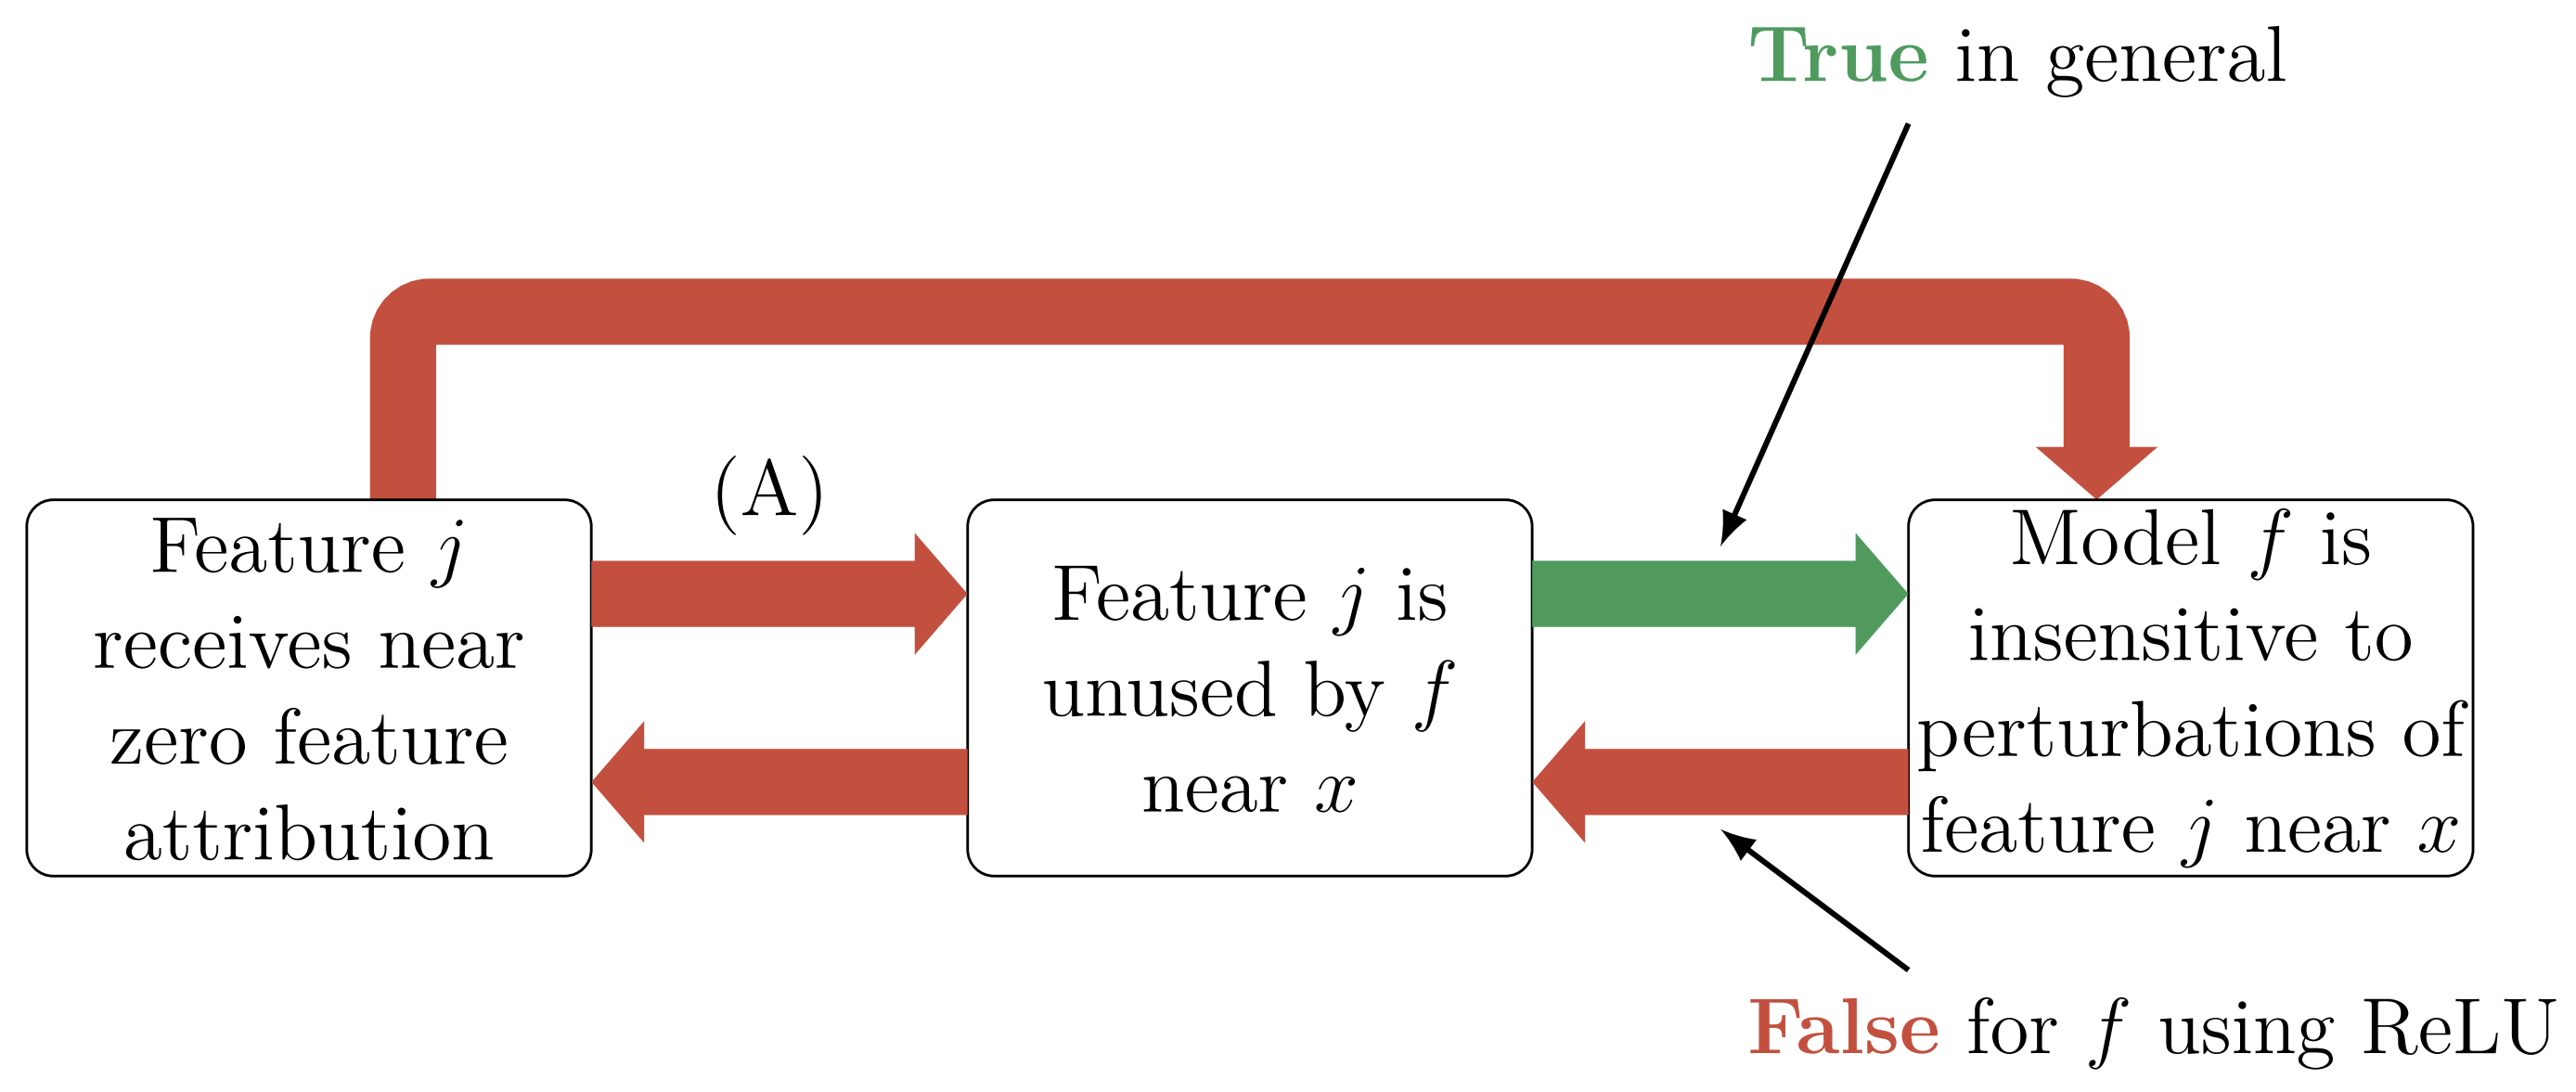
\includegraphics[width=0.75\linewidth]{figure-files/overview.png}
\caption{
Red arrows indicate false implications for \completename{} and \additivename{} \fieldmethodnames{}, which follows from \cref{fact:oracle-hypothesis}.
Implication (A) is a standard belief in the literature for \fielddefnames{},
%
but we show it is false in general.
}
\label{fig:intgrad-spurious-implications}
\end{figure}

%
%
%
%
%
%

%
%
%
%
%
%
%

%
%
%
%
%
%
%

%
%
%
%
%
%
%
%
%
